% Latex template: mahmoud.s.fahmy@students.kasralainy.edu.eg
% For more details: https://www.sharelatex.com/learn/Beamer

\documentclass[aspectratio=1610]{beamer}					% Document class

\setbeamertemplate{footline}[text line]{%
  \parbox{\linewidth}{\vspace*{-8pt}Interferon-$\gamma$ induction of GBP5 in HeLa cells \hfill\insertshortauthor\hfill\insertpagenumber}}
\setbeamertemplate{navigation symbols}{}

\usepackage[english]{babel}				% Set language
\usepackage[utf8x]{inputenc}			% Set encoding

\mode<presentation>						% Set options
{
  \usetheme{default}					% Set theme
  \usecolortheme{default} 				% Set colors
  \usefonttheme{default}  				% Set font theme
  \setbeamertemplate{caption}[numbered]	% Set caption to be numbered
}

% Uncomment this to have the outline at the beginning of each section highlighted.
%\AtBeginSection[]
%{
%  \begin{frame}{Outline}
%    \tableofcontents[currentsection]
%  \end{frame}
\usepackage{graphicx}					% For including figures
\usepackage{booktabs}					% For table rules
\usepackage{hyperref}	
\usepackage{tikz-network}				% For cross-referencing
\usepackage[absolute,overlay]{textpos}
\usepackage{bm}
\usepackage[font=small,labelfont=bf]{caption}				% For cross-referencing

\title{Interferon-$\gamma$ induction of GBP5 in HeLa cells}	% Presentation title
\author{Clayton W. Seitz}								% Presentation author
\date{\today}									% Today's date	

\begin{document}

% Title page
% This page includes the informations defined earlier including title, author/s, affiliation/s and the date
\begin{frame}
  \titlepage
\end{frame}


% The following is the most frequently used slide types in beamer
% The slide structure is as follows:
%
%\begin{frame}{<slide-title>}
%	<content>
%\end{frame}

\begin{frame}{The principle of Interferon-$\gamma$ induced transcriptional memory}
\begin{figure}
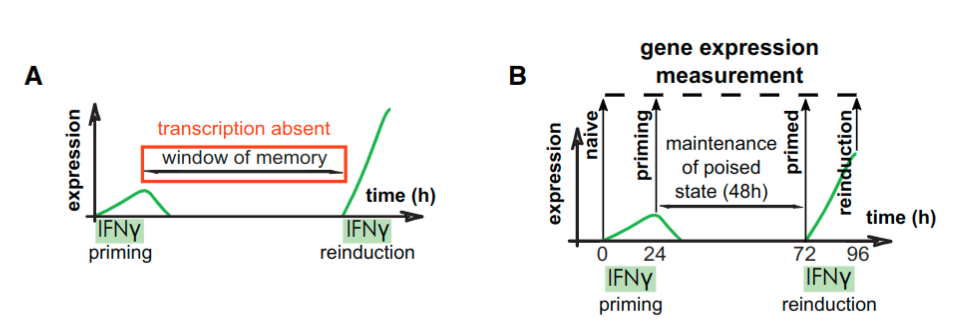
\includegraphics[width=14cm]{Memory.png}
\caption{}
\end{figure}

Siwek et al. \textit{Activation of Clustered IFNg Target Genes Drives Cohesin-Controlled Transcriptional Memory}. Molecular Cell 2020

\end{frame}


\begin{frame}{Rare HeLa cell GBP5 expression @ 24h after reinduction with IFN-$\gamma$}
Show tiled images
Needs validation in another cell line
\end{frame}

\begin{frame}{Rare HeLa cell GBP5 expression @ 24h after reinduction with IFN-$\gamma$}
\begin{figure}
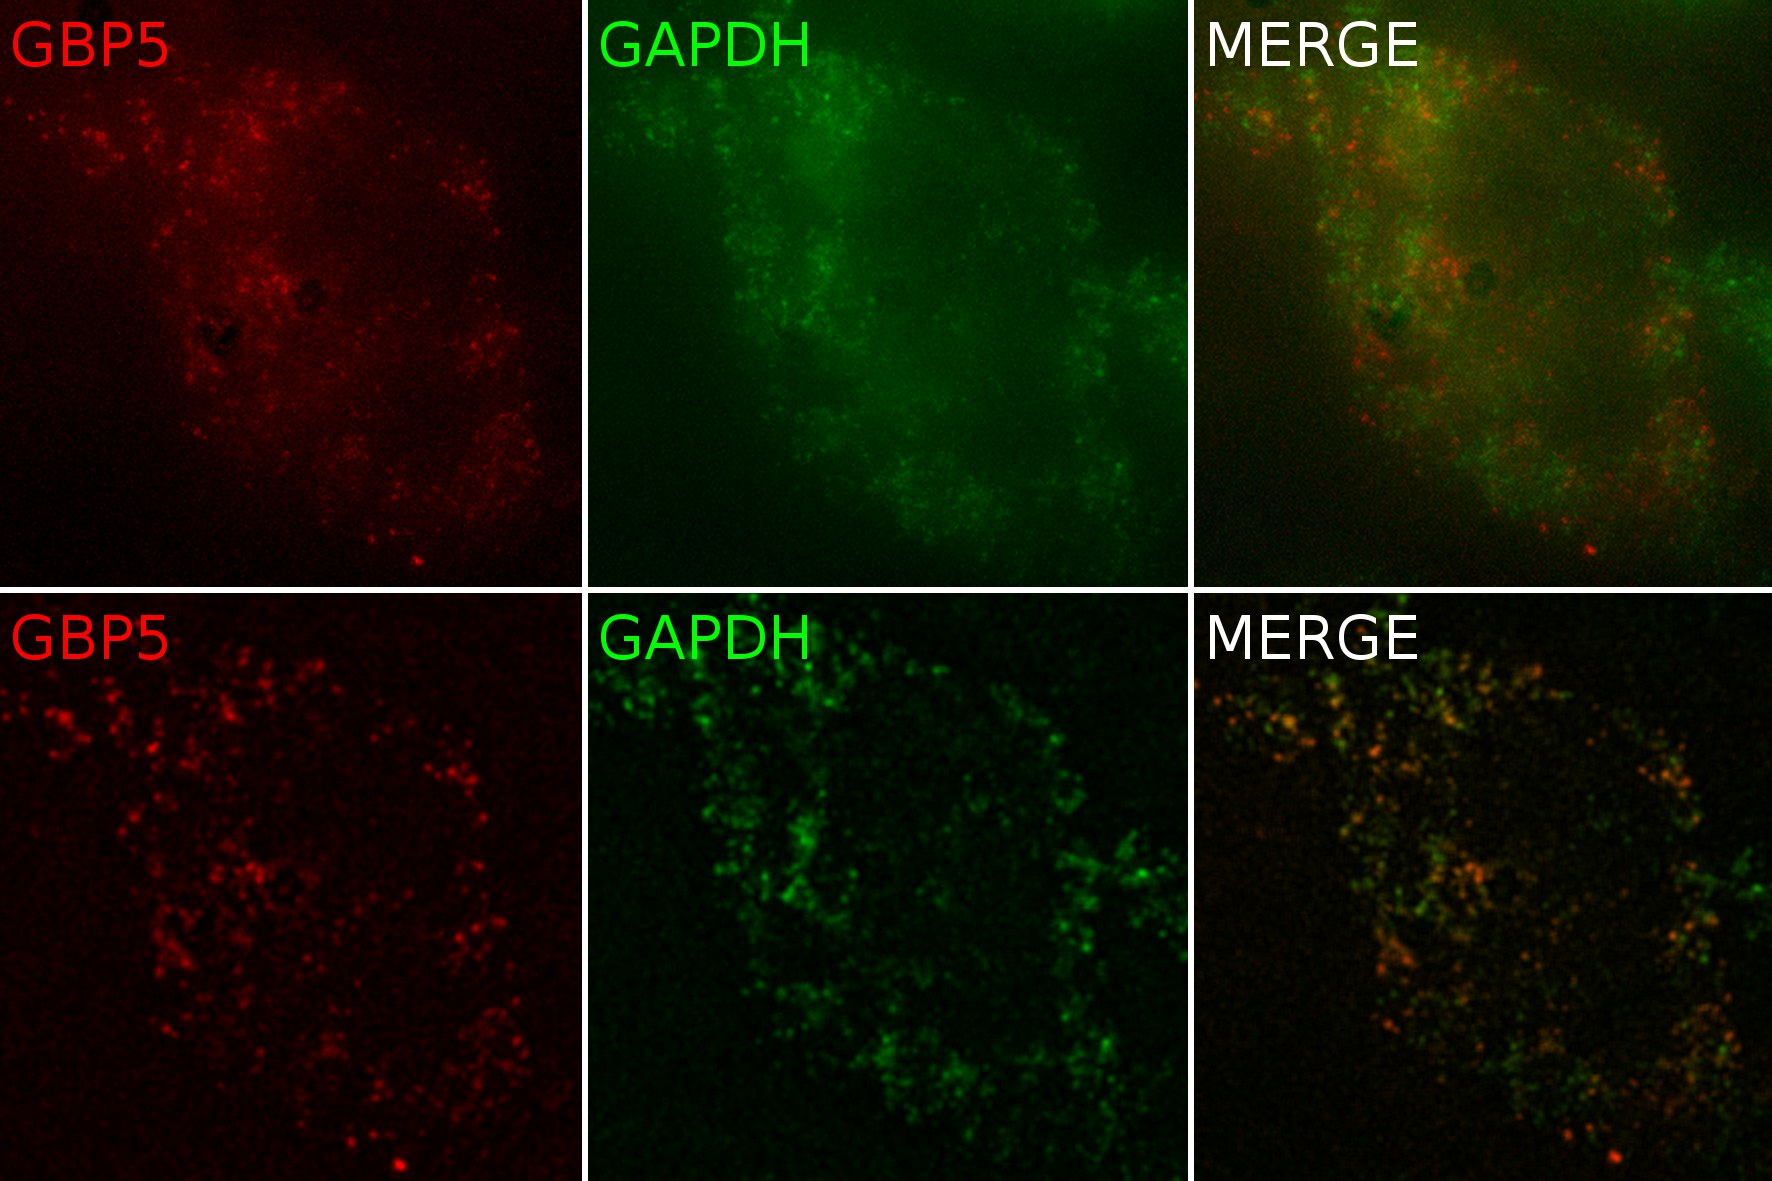
\includegraphics[width=12cm]{Stains.png}
\end{figure}
\end{frame}

\begin{frame}{Intensity histogram for rare GBP5 expression}
\begin{figure}
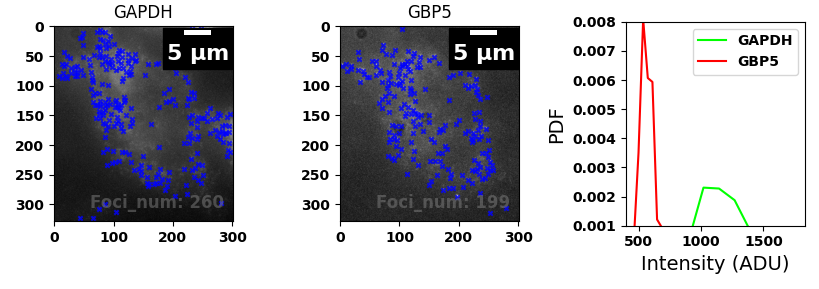
\includegraphics[width=14cm]{Detection.png}
\end{figure}
\begin{itemize}
\item \textcolor{red}{Very few ($\sim 1\%$)} reinduced cells express GBP5, but those that do express at high levels (relative to GAPDH)
\item Control sample shows little to no GBP5 expression
\end{itemize}
\end{frame}

\begin{frame}{Comments on ergodicity of transcription}
\begin{figure}
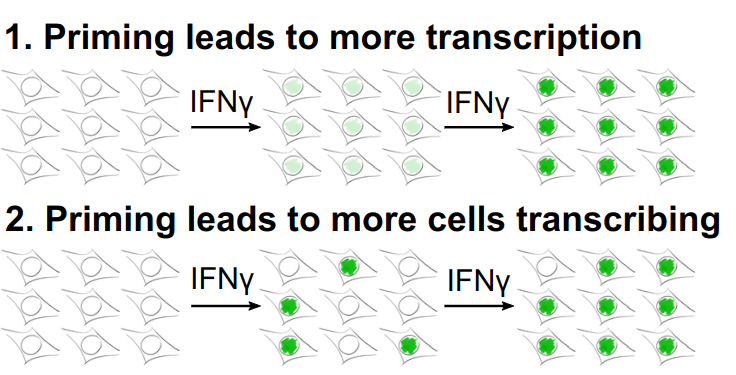
\includegraphics[width=10cm]{Ergodic.png}
\end{figure}
\begin{itemize}
\item RNA flow cannot apply to non-ergodic systems (yet ergodicity is often assumed)
\item Previous work suggests that IFN-$\gamma$ induces epigenetic changes at the GBP5 locus
\item What is the epigenetic change? Is the epigenetic change all or nothing?
\end{itemize}
\vspace{0.1in}


\end{frame}

\begin{frame}{Epigenetic changes at GBP genes after IFN-$\gamma$ treatment}
Siwek et al. \textit{Activation of Clustered IFNg Target Genes Drives Cohesin-Controlled Transcriptional Memory}. Molecular Cell 2020
\begin{figure}
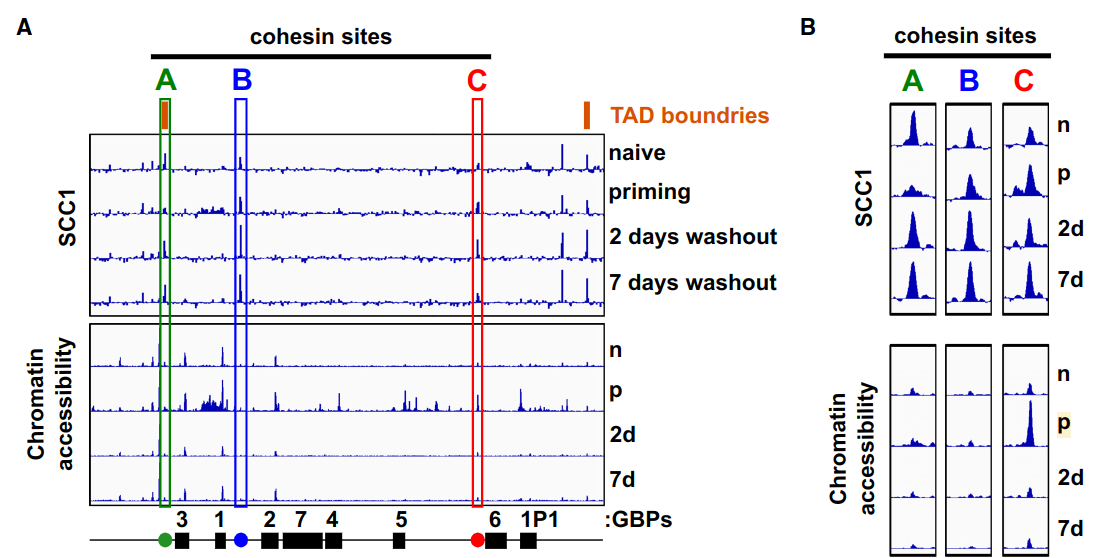
\includegraphics[width=12cm]{Epigenetic.png}
\end{figure}
\end{frame}

\begin{frame}{STORM imaging of H2B}
\begin{figure}
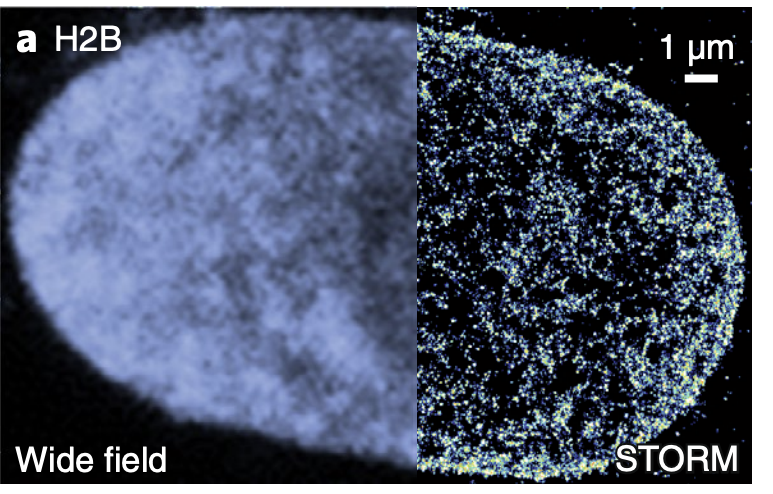
\includegraphics[width=12cm]{STORM.png}
\end{figure}
Lakadamyali et al. \textit{Visualizing the genome in high resolution
challenges our textbook understanding}. Nature Methods 2020
\end{frame}

\begin{frame}{Working principle of dSTORM}
\begin{figure}
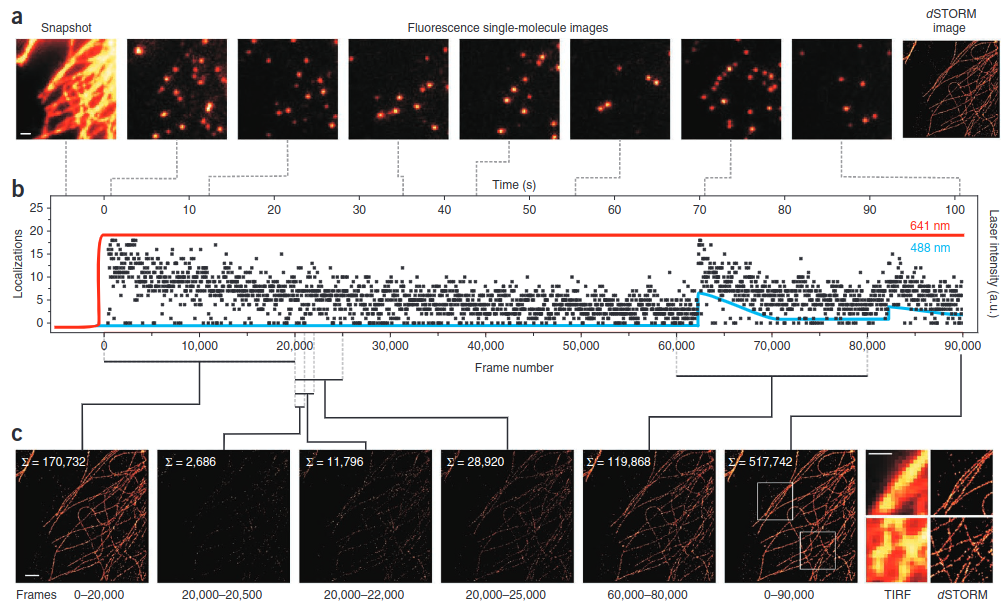
\includegraphics[width=13cm]{dSTORM2.png}
\end{figure}
\end{frame}

\begin{frame}{Details on STORM timing setup}
\begin{figure}
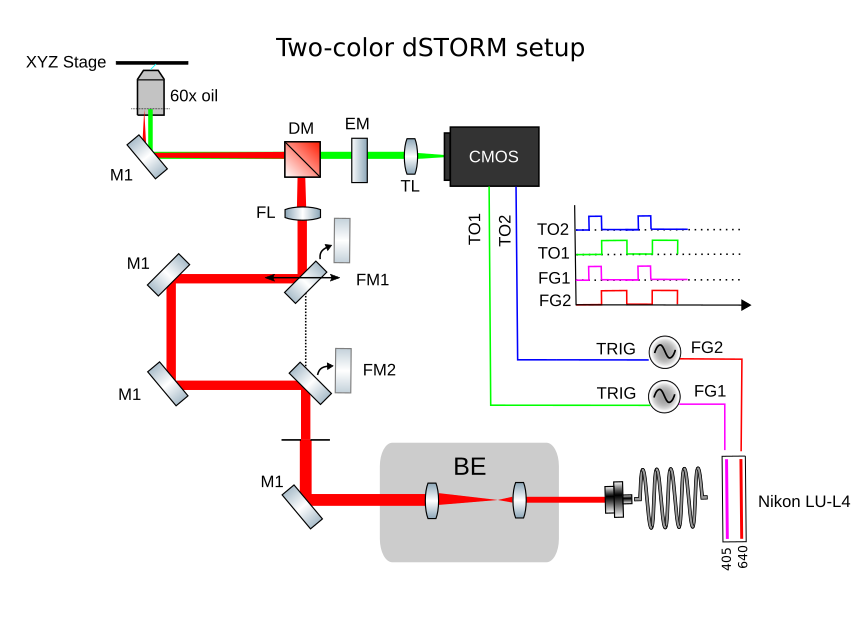
\includegraphics[width=12cm]{dSTORM.png}
\end{figure}
\end{frame}

\begin{frame}{Using STORM to measure epigenetic changes}
But it is difficult to study epigenetic changes at a single gene, without additional methods e.g., DNA FISH + STORM microscopy. Let's talk about STORM
\end{frame}

\end{document}